% This is "sig-alternate.tex" V2.0 May 2012
% This file should be compiled with V2.5 of "sig-alternate.cls" May 2012
%
% This example file demonstrates the use of the 'sig-alternate.cls'
% V2.5 LaTeX2e document class file. It is for those submitting
% articles to ACM Conference Proceedings WHO DO NOT WISH TO
% STRICTLY ADHERE TO THE SIGS (PUBS-BOARD-ENDORSED) STYLE.
% The 'sig-alternate.cls' file will produce a similar-looking,
% albeit, 'tighter' paper resulting in, invariably, fewer pages.
%
% ----------------------------------------------------------------------------------------------------------------
% This .tex file (and associated .cls V2.5) produces:
%       1) The Permission Statement
%       2) The Conference (location) Info information
%       3) The Copyright Line with ACM data
%       4) NO page numbers
%
% as against the acm_proc_article-sp.cls file which
% DOES NOT produce 1) thru' 3) above.
%
% Using 'sig-alternate.cls' you have control, however, from within
% the source .tex file, over both the CopyrightYear
% (defaulted to 200X) and the ACM Copyright Data
% (defaulted to X-XXXXX-XX-X/XX/XX).
% e.g.
% \CopyrightYear{2007} will cause 2007 to appear in the copyright line.
% \crdata{0-12345-67-8/90/12} will cause 0-12345-67-8/90/12 to appear in the copyright line.
%
% ---------------------------------------------------------------------------------------------------------------
% This .tex source is an example which *does* use
% the .bib file (from which the .bbl file % is produced).
% REMEMBER HOWEVER: After having produced the .bbl file,
% and prior to final submission, you *NEED* to 'insert'
% your .bbl file into your source .tex file so as to provide
% ONE 'self-contained' source file.
%
% ================= IF YOU HAVE QUESTIONS =======================
% Questions regarding the SIGS styles, SIGS policies and
% procedures, Conferences etc. should be sent to
% Adrienne Griscti (griscti@acm.org)
%
% Technical questions _only_ to
% Gerald Murray (murray@hq.acm.org)
% ===============================================================
%
% For tracking purposes - this is V2.0 - May 2012

\documentclass{sig-alternate}
\newtheorem{definition}{Definition}
\usepackage{url}
\usepackage{soul,color}
\usepackage{anyfontsize}
\begin{document}
\title{Capturing policies for fine-grained access-control}
% --- Author Metadata here ---
\conferenceinfo{HotMobile'16}{February 23-24, 2016, St. Augustine, Florida, USA}
\CopyrightYear{2016} % Allows default copyright year (20XX) to be over-ridden - IF NEED BE.
%\crdata{0-12345-67-8/90/01}  % Allows default copyright data (0-89791-88-6/97/05) to be over-ridden - IF NEED BE.
% --- End of Author Metadata ---
%
% You need the command \numberofauthors to handle the 'placement
% and alignment' of the authors beneath the title.
%
% For aesthetic reasons, we recommend 'three authors at a time'
% i.e. three 'name/affiliation blocks' be placed beneath the title.
%
% NOTE: You are NOT restricted in how many 'rows' of
% "name/affiliations" may appear. We just ask that you restrict
% the number of 'columns' to three.
%
% Because of the available 'opening page real-estate'
% we ask you to refrain from putting more than six authors
% (two rows with three columns) beneath the article title.
% More than six makes the first-page appear very cluttered indeed.
%
% Use the \alignauthor commands to handle the names
% and affiliations for an 'aesthetic maximum' of six authors.
% Add names, affiliations, addresses for
% the seventh etc. author(s) as the argument for the
% \additionalauthors command.
% These 'additional authors' will be output/set for you
% without further effort on your part as the last section in
% the body of your article BEFORE References or any Appendices.

\numberofauthors{8} %  in this sample file, there are a *total*
% of EIGHT authors. SIX appear on the 'first-page' (for formatting
% reasons) and the remaining two appear in the \additionalauthors section.
%
\author{
% You can go ahead and credit any number of authors here,
% e.g. one 'row of three' or two rows (consisting of one row of three
% and a second row of one, two or three).
%
% The command \alignauthor (no curly braces needed) should
% precede each author name, affiliation/snail-mail address and
% e-mail address. Additionally, tag each line of
% affiliation/address with \affaddr, and tag the
% e-mail address with \email.
%
% 1st. author
\alignauthor Prajit Kumar Das\\
\affaddr{University of Maryland, Baltimore County}\\
%\affaddr{Baltimore, MD, USA}\\
\email{prajit1@umbc.edu}
% 2nd. author
\alignauthor Sandeep Narayanan\\
\affaddr{University of Maryland, Baltimore County}\\
%\affaddr{Baltimore, MD, USA}\\
\email{sand7@umbc.edu}
% 3rd. author
\alignauthor Stanislav Bobovych\\
\affaddr{University of Maryland, Baltimore County}\\
%\affaddr{Baltimore, MD, USA}\\
\email{sb9@umbc.edu}
\and  % use '\and' if you need 'another row' of author names
% 4th. author
\alignauthor Anupam Joshi\\
\affaddr{University of Maryland, Baltimore County}\\
%\affaddr{Baltimore, MD, USA}\\
\email{joshi@umbc.edu}
% 5th. author
\alignauthor Nilanjan Banerjee\\
\affaddr{University of Maryland, Baltimore County}\\
%\affaddr{Baltimore, MD, USA}\\
\email{nilanb@umbc.edu}
% 6th. author
\alignauthor Ryan Robucci\\
\affaddr{University of Maryland, Baltimore County}\\
%\affaddr{Baltimore, MD, USA}\\
\email{robucci@umbc.edu}
}
% \and  % use '\and' if you need 'another row' of author names
% 7th. author
% \alignauthor Ting Zhu\\
% \affaddr{University of Maryland, Baltimore County}\\
%\affaddr{Baltimore, MD, USA}\\
% \email{zt@umbc.edu}
% 8th. author
% \alignauthor Tim Finin\\
% \affaddr{University of Maryland, Baltimore County}\\
%\affaddr{Baltimore, MD, USA}\\
% \email{finin@umbc.edu}
% }
% There's nothing stopping you putting the seventh, eighth, etc.
% author on the opening page (as the 'third row') but we ask,
% for aesthetic reasons that you place these 'additional authors'
% in the \additional authors block, viz.
\additionalauthors{Additional authors: Ting Zhu (University of Maryland, Baltimore County,
email: {\texttt{zt@umbc.edu}}) and Tim Finin (University of Maryland, Baltimore County, email: {\texttt{finin@umbc.edu}}).}
\date{19 July 2015}
% Just remember to make sure that the TOTAL number of authors
% is the number that will appear on the first page PLUS the
% number that will appear in the \additionalauthors section.
\maketitle
%{\Large %Remove comment '%' to get a 'Large' font introduction section and abstract
\begin{abstract}
The number of mobile devices in the world surpassed the number of personal computers in 2010. Mobile devices now carry sensitive personal data, captured through sensors on the phone, as well as confidential corporate data through work emails and apps. As a result, they have become lucrative targets for attackers and the privacy and security of these devices have become a vital issue. Existing access control mechanisms on these devices, which mostly rely on a one-time permission grant, are too restrictive and inadequate. Such mechanisms are incapable of controlling contextual or custom app-data flows. In this paper we focus on this scenario and show how data leakages may occur due to developer inadequacy and a lack of proper checks for such leakages. We describe a design flaw in the Android permission verification mechanism and a way to capture such a vulnerability on a user's mobile device. We also show a mechanism of injecting such a vulnerability into any app.
\end{abstract}
% A category with the (minimum) three required fields
\category{D.4.6}{Operating Systems}{Security and Protection}[Access Controls]
%\terms{Access Control, Mobile privacy and security}
\keywords{Access Control, Android Content Providers, Permission Control}

\section{Introduction}
\label{intro}
Mobile devices have become ubiquitous due to its low cost and Android is the biggest player in the market. Latest reports from Google boasts of more than a billion active 30 day user~\cite{Engadget_market_share}. According to the International Data Corporation's Worldwide Quarterly Mobile Phone Tracker report Android has a 85\% market share in the smartphone category. Apps from the Google Play Store and a variety of other app-stores like Amazon App Store and Samsung Galaxy Apps provide a plethora of ways through which Android users can get their apps~\cite{Online_App_Stores}. According to Statista~\cite{Android_app_number}, as of July 2015, there are more than 1.6 million android apps in the Google Play Store. 

The proliferation of smartphones has led to the popularity of the BYOD(Bring-Your-Own-Device) paradigm, whereby users' use their personal devices for corporate purposes. Naturally, this creates a greater need to ensure strong access control mechanisms for the data on such devices. In certain domains the access control needs are of a critical nature. For example in the category of Medical and Health \& fitness apps it is essential that user data and if being used in hospitals, corporate data security be maintained to the utmost level. Hospitals today use various hardware devices that are smart enough to communicate with smartphones and may even contain sensitive medical data. In addition to that android apps are capable of collecting a huge amounts of data about the smartphone user, often without the knowledge of the user. 

There have been multiple attempts at achieving the goal of properly managing access control on mobile (Android) devices. Efforts have been made by the open source community through the XPrivacy project (needs a rooted phone), the Privacy Guard project (available on Cyanogenmod, a custom Android ROM), the PDroid application (needs a rooted device). Research project by Conti et. al.~\cite{conti2011crepe}(CRePe), Enck et al.~\cite{enck2010taintdroid}(TaintDroid) and Jagtap et al.~\cite{Jagtap2011Privacy}(Preserving Privacy in Context-Aware Systems) have made similar efforts. CRePE described a system where security policy enforcement was carried out based on context of the smart phone. TaintDroid was a research effort where the data flow on an Android device was studied to figure out when sensitive data left the system via an untrusted application. The work of Jagtap et al.~\cite{Jagtap2011Privacy} focused on constraining data flow in a context-aware system using a policy-based framework. A related work by Ghosh et al.~\cite{ghosh2012privacy} used a similar policy driven approach to constrain application permissions based on context. A %Given the abundance of works in the access control area, its understandable that the latest version of Android (Marhsmallow), embraced a new permission model. Android now boasts of a runtime, on-demand permission acquisition model, similar to iOS, the other leading smartphone platform. Such a change, although welcome, still remains inadequate with respect to context based data flow control. Android has attempted to make the transition for its developers and users simple by grouping the control into logical groups but it still leaves a lot to desire.

In this paper we focus on a custom permissions created by app developers. These permissions are there to protect the app developers data on their own content providers. It is advised by Google that if an app developer creates a content provider for allowing access to it's own data, they should create a permission to control access to it. However, this requirement is not a stringent one and one might simply ignore creating such a permission.

%Some of them include Blood glucose monitoring system[5], Blood pressure monitor[6], Heart monitor[7], Fitness accessories like Fitbit, Breathalyzer[4] etc. All these accessories have an associated Android application which interacts with the physical device, process the data, display it and stores relevant information. Another category of applications are those used by hospitals and its employees to manage information about the patients, doctors etc. The important point is that all these sensitive information are being received, processed, stored and possibly updated to cloud storage by these applications. The fact that personal and sensitive data is handled by these devices presents a potential security risk. With more than 1.6 million apps to choose from, let alone a layman user, even a computer expert will have difficulty to understand what are benign and what are malicious. One of the most traditional ways to look at this problem is to use signature based malware detection, in which once a malware application is detected, signature will be created once and the signatures are updated to a common database. Any future appearance of the same malware would be detected using these signatures. The classical problem with this approach is the occurrence of mutating malwares which changes it’s signature every time it is spread and it inability to detect future similar attacks. Apart from this Android apps has issues on its own. One of the main problem is the high volatility of the app markets. Since unlike Apple store, Google play store is not verified and hence new applications becomes available and taken out quite frequently. Yet another issue is repackaging popular application with malware. Often these repackaged applications are uploaded to other local App-stores where the original application is not available. Hence we require a faster and dynamic setup to detect unsafe or rather potentially unsafe applications. [Paper to be referred Dr B]Even though not totally accurate, there are some intuitions which we can utilize from the meta-data available with each application. The different meta-data available with each of these applications include App description, Permissions required, Number of downloads, Broad Application categories etc. As an example of our intuition let us take the case of “brightestlight” application, which is available in Google Play Store. The description of the application says that it is a flash light app, which shows some unobtrusive Ads. But on analyzing the Permissions required, we can see that the application requests permissions for location (accurate GPS and approximate network based), file manipulation (read, modify and delete USB storage), camera (curiously it includes auto-focus permission) etc. This does seem suspicious. But still we cannot say that the application is unsafe, rather we need further investigation. 

\section{Related Work}
\label{RelatedWork}
\hl{
Playdrone : Crawls Playstore- how playstore evolved - source code analysis of library usage - similar app detection-secret authentication key storage (can be found by decompilation)
(1) native libraries are heavily used by popular Android applications, limiting the benefits of Java portability and the ability of Android server overloading systems to run these applications, (2) 25\% of Google Play is duplicative application content, and (3) Android applications contain thousands of leaked secret authentication keys which

Andradar : First, we can discover malicious applications in alternative markets, second, we can expose app distribution strategies used by malware developers, and third, we can monitor how different markets react to new malware. To identify and track malicious apps still available in a number of alternative app markets.

Android Security : discuss the Android security enforcement mechanisms, threats to the existing security enforcements and related issues, malware growth timeline between 2010 and 2014, and stealth techniques employed by the malware authors, in addition to the existing detection methods. This review gives an insight into the strengths and shortcomings of the known research methodologies and provides a platform, to the researchers and practitioners, toward proposing the next-generation Android security, analysis, and malware detection techniques.

ANDRUBIS:, a fully automated, publicly available and comprehensive analysis system for Android apps. ANDRUBIS combines static analysis with dynamic analysis on both Dalvik VM and system level, as well as several stimulation techniques to increase code coverage. 

changes in the malware threat landscape and trends amongst goodware developers. Dynamic code loading, previously used as an indicator for malicious behavior, is especially gaining popularity amongst goodware App analysis for astma!!

App behavoir against description CHABADA tool clustering apps by description topics, and identifying outliers
by API usage within each cluster, our CHABADA approach effectively
identifies applications whose behavior would be unexpected
given their description.
Recommendations for android eco system}
\section{System Overview}
\label{overview}

Heimdall has two components: the first is an app installed on a user's mobile device and the second is a Web service that receives install, uninstall and update notifications when these events occur on the device. Upon notification, the server processes all heuristics that apply to the app and generates a set of actions for a system administrator. At this point the system administrator can take an appropriate action based on the detected threat level. Our present prototype, includes a simple content provider heuristic that estimates the impact of a vulnerability. The only solution that is possible, at the moment, is to uninstall the app and that notification is then sent back to the user's device automatically.

\begin{figure}[tb]
	\centering
	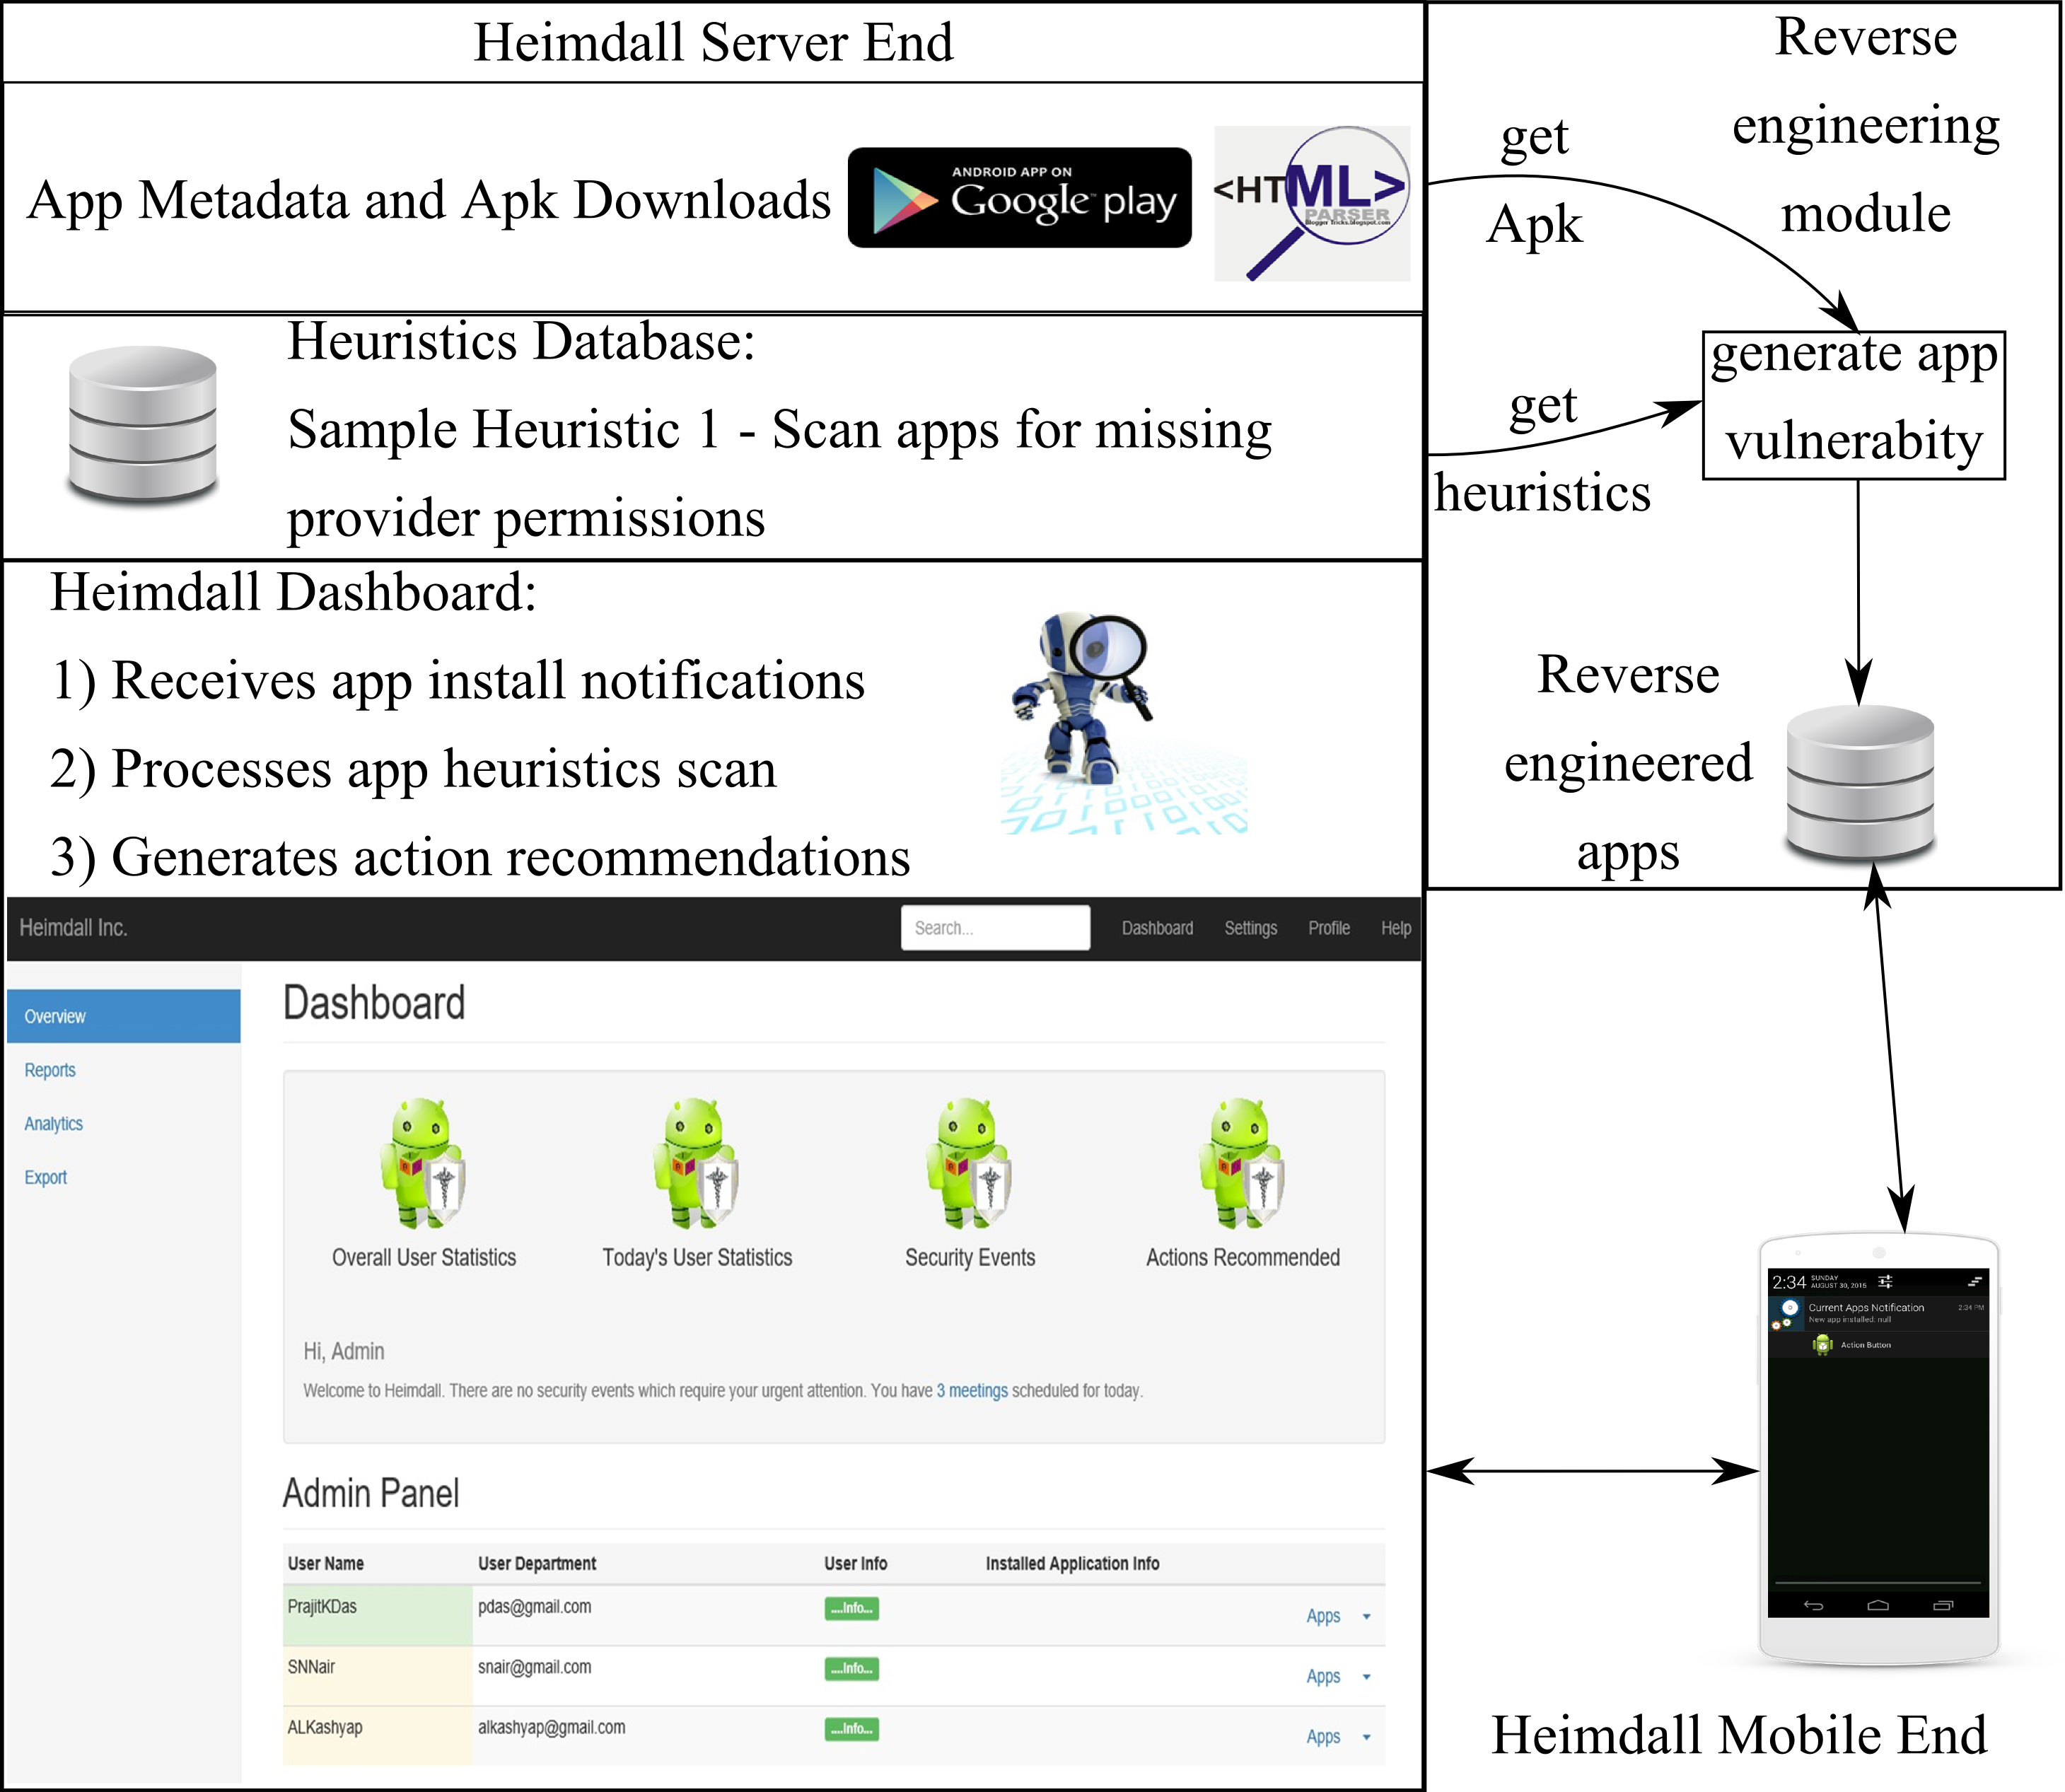
\includegraphics[width=\columnwidth]{images/architecture}
	\caption{System Overview}
	\label{fig:arch}
\end{figure}

Heimdall server has two additional capabilities. The first is to generate reverse engineered apps that we then test on the mobile devices. The reverse engineering process removes any provider associated permission and ensures that the ``exported'' tag for the provider is set to true. The second capability is to scan for missing provider permissions for known apps. For this purpose we downloaded about 1500 apps from the Google Play Store and then we use the \footnote{apktool~\url{https://ibotpeaches.github.io/Apktool/}} package to decompile the Android application packages (apks) and parse the manifest files to determine if any of the app's provider is missing the permission association. Naturally, as we include more heuristics, Heimdall will become capable of detecting much more such vulnerability.

%\begin{figure}[tb]
	%\centering
	%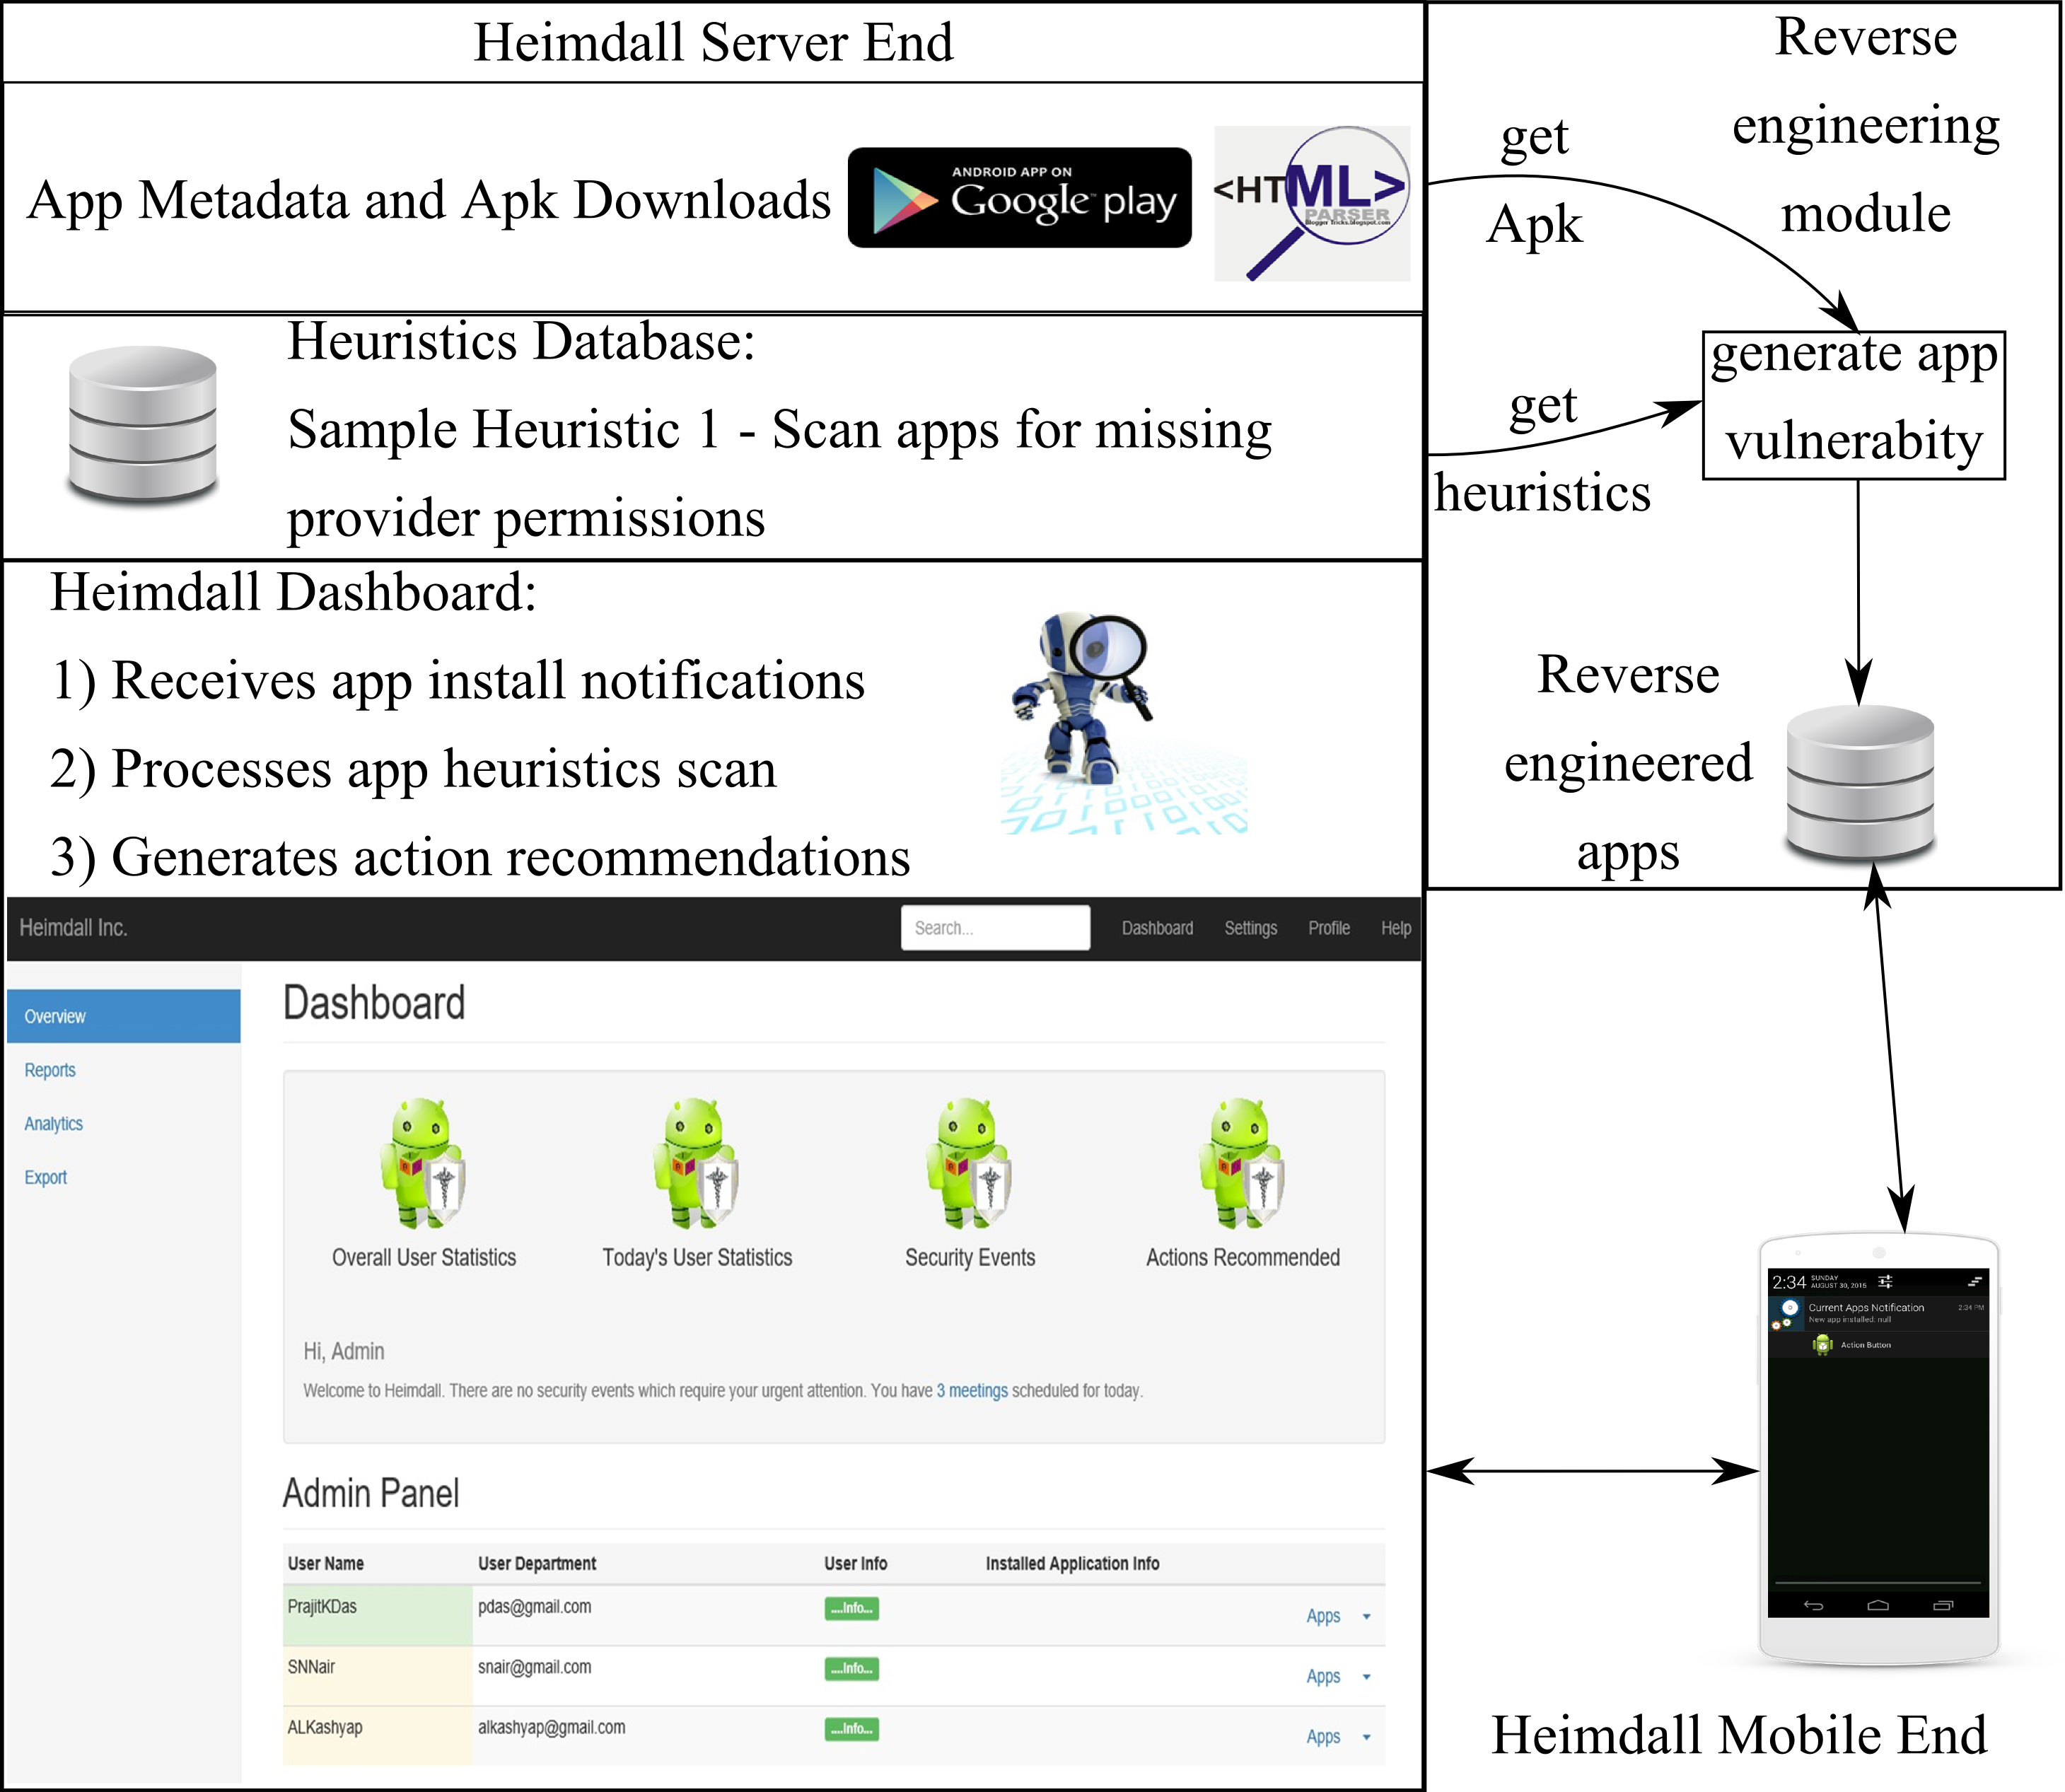
\includegraphics[width=\columnwidth]{images/architecture}
	%\caption{System Architecture}
	%\label{fig:arch}
%\end{figure}

\section{Vulnerability Description}
\label{vuln}
\noindent
In Android, a content provider is a data repository for an application, which offers a consistent and standard interface for secure data access. It is mainly used for sharing data across applications and hence need to be protected with adequate permissions to prevent inadvertent data leakages. Google's Android documentation describes two possible scenarios. The first scenario states that data from a provider that specifies no permissions should not be accessible from other apps, while the second scenario states a conflicting view as quoted below.
\begin{itemize}
 \item ``[...] If a provider's application doesn't specify any permissions, then other applications have no access to the provider's data. However, components in the provider's application always have full read and write access, regardless of the specified permissions.''~\footnote{Error in specification~\url{http://developer.android.com/guide/topics/providers/content-provider-basics.html#Permissions}}
 \item ``[...] All applications can read from or write to your provider, even if the underlying data is private, because by default your provider does not have permissions set. To change this, set permissions for your provider in your manifest file, using attributes or child elements of the <provider> element. You can set permissions that apply to the entire provider, or to certain tables, or even to certain records, or all three.''~\footnote{Correct specification~\url{http://developer.android.com/guide/topics/providers/content-provider-creating.html#Permissions}}
\end{itemize}
\begin{center}
	\begin{table}
		\label{tableErrors}
		\begin{tabular}{ | p{2.5cm} | p{2.5cm} | p{2cm} | }
			\hline
			\textbf{Content Provider app} & \textbf{Content accessing app} & \textbf{Remark} \\
			\hline \hline
			No permission associated with provider & No permission used & \textcolor[rgb]{1,0,0}{\textbf{Potential data leakage}} \\
			\hline
			Permission associated with provider & No permission used & Permission denied \\
			\hline
			Permission associated with provider & Permission used & Ideal scenario \\
			\hline
			No permission associated with provider & Permission used & No error \\
			\hline
		\end{tabular}
		\caption{Scenario when data leakage may happen}
	\end{table}
\end{center}
\noindent
Unfortunately, we found the first statement to be untrue. Table~\ref{tableErrors} lists the various scenarios and points out when a content provider app is not associated with a permission we may have data leakage. This happens because Android does not verify that each provider has an associated permission. There is one more condition required for this vulnerability to open up the provider to potential attacks and that is the exported setting to be set as true in the Manifest file for the provider app, as shown in code Listing~\ref{providerCode}. Possible solutions to mitigate this issue would require, either a change in how Android handles content provider access control or a change in the app developer's code.

\begin{lstlisting}[caption={Provider exported tag set as true},label={providerCode},language=XML]
...
<provider
	android:name="contentProviderName"
	android:authorities="authorityName"
	android:exported="true">
...
\end{lstlisting}

Such a vulnerability can also be created deliberately. As shown in the work by Zhou et. al.~\cite{Zhou2012MalwareGenomeProject} app repackaging is one of the most common techniques for android malware creation, we show that it is possible through a simple change in code to introduce such a vulnerability in any app. There are some obvious ways to check for such manipulations and top developers in the Google Play Store usually do include such checks. However, these checks are not part of the android framework or operating systems and therefore a repackaged app can be used to fool users into installing a rogue application and allow their data to be stolen.

\section{Evaluation}
\label{eval}
\noindent
We have discussed a potential loophole in Android's custom provider data flow, in this paper. We are going to demonstrate four possible scenarios for this loophole through our experiments. In each case, the vulnerability either already exists in the app or it was introduced by us. In scenario 1 we have an app that has the vulnerability and does nothing to protect itself and we know the exact URI call to access the content provider. Scenario 2 is where the app uses certificate key signatures to detect the reverse engineering and blocks any attempt to start the app itself. Scenario 3 is where the app does not crash at all and works like a normal app. However, when one tries to access a component of the app like a content provider, the app includes custom access control checks. Scenario 4 is still under investigation, but this is the case  where an app's URI string can be fully obtained by a combination of parsing the Manifest file and guess work. In order to demonstrate this problem we built a proof-of-concept(PoC). All our experiments were ran on a LG Nexus 5 device with Android Marshmallow 6.0 installed on it.

\subsection{Scenario 1: Vulnerability with complete knowledge}
In our PoC, we have an app(COMMAND) that has an exported content provider. We created another app(Parser) that is capable of accessing the content provider. We use two different application package sets and observe the results. The first set contains the COMMAND app without any permission specification and Parser app without any permission request. The second set contains the COMMAND app with permission specification and association with the content provider that was created. It also includes the Parser app with a request for the permission that was created by COMMAND.

\subsubsection{PoC case 1 for permission control} COMMAND has associated permission, Parser has requested said permission. We see in Figure~\ref{fig:bothHavePerm} that, in this case there are no errors and we are able to make a sample query to the content provider.
\subsubsection{PoC case 2 for permission control} COMMAND has no associated permission, Parser has not requested said permission. We see in Figure~\ref{fig:neitherHavePerm} that, in this case there are no errors and we are able to make a sample query to the content provider. We propose that there should be a check in such a case to ensure that data access is to be allowed or denied. At present this does not happen and app developers resort to individual techniques to protect their data.
\begin{figure}
\centering
\begin{minipage}{.45\columnwidth}
	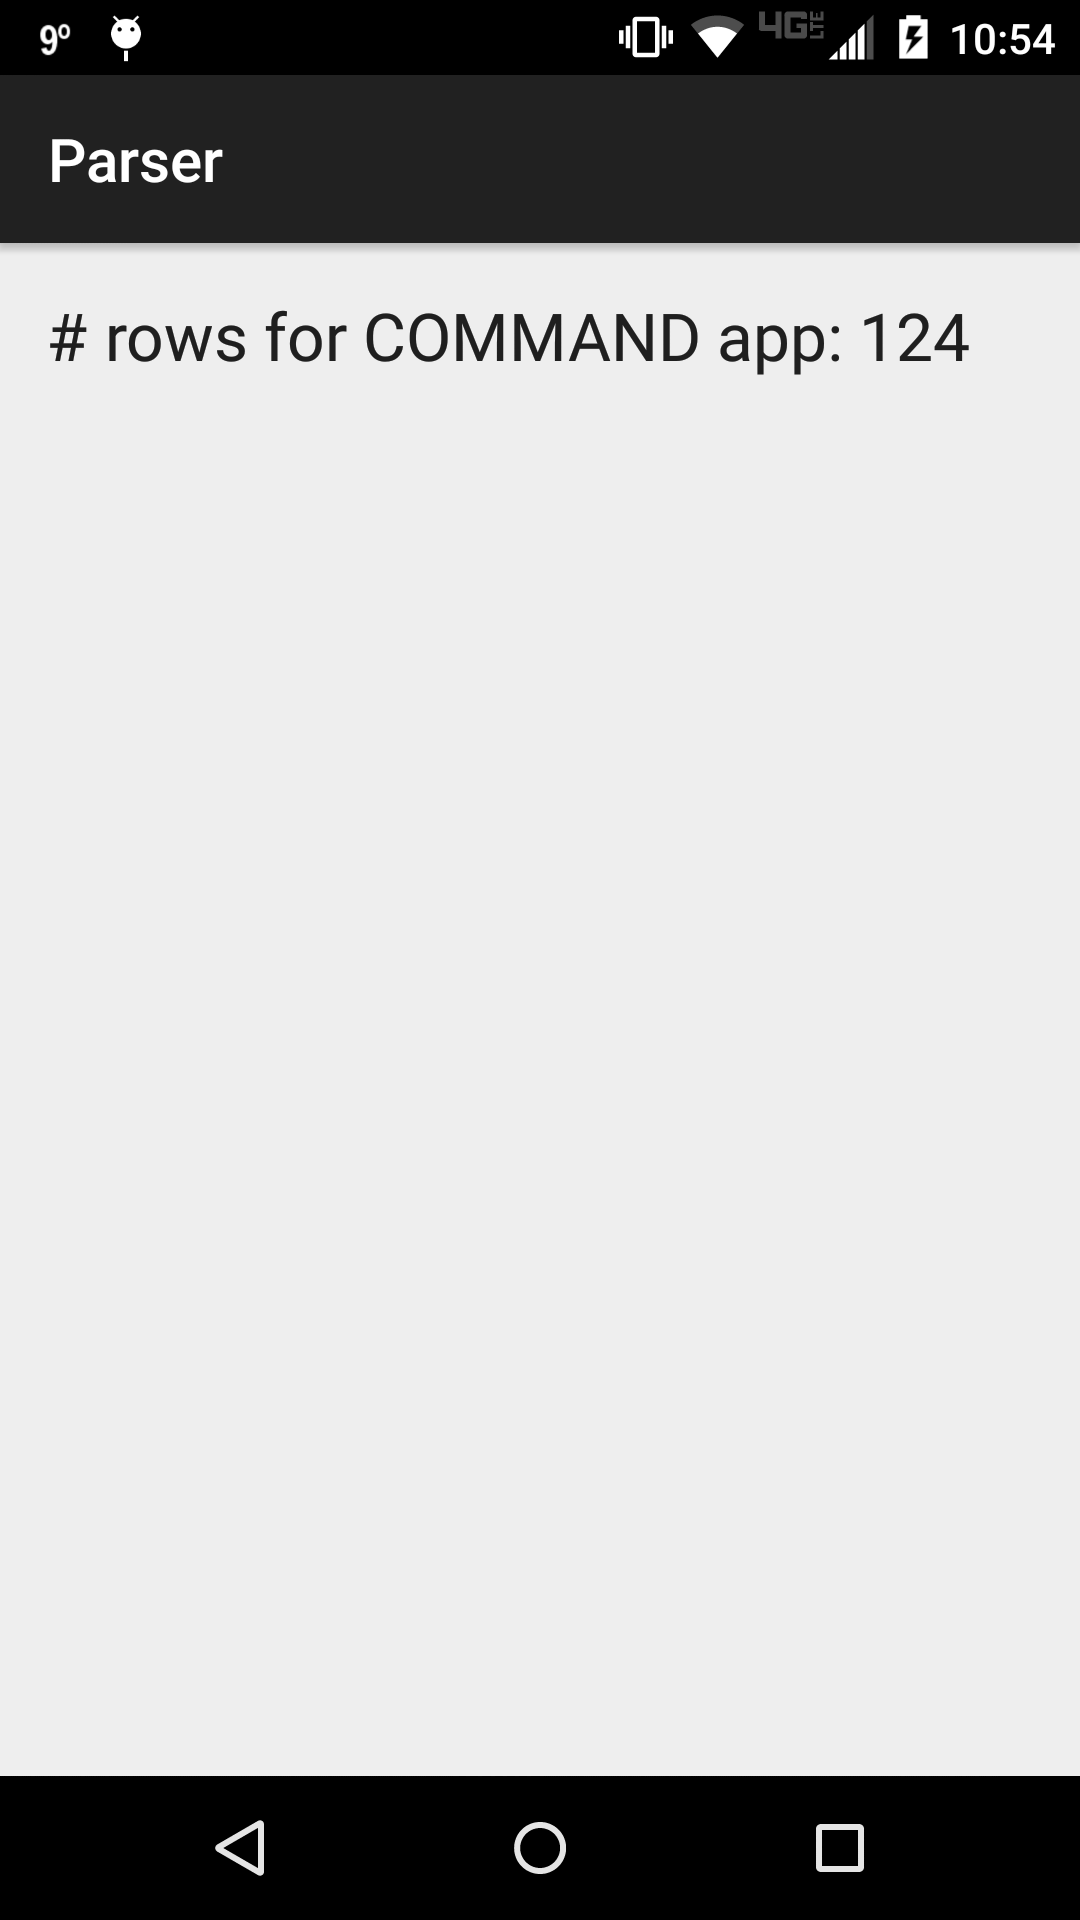
\includegraphics[width=\columnwidth,scale=0.5]{images/bothHavePerm}
	\caption{Android content provider accessed with permission}
	\label{fig:bothHavePerm}
\end{minipage}
\hspace{.05\linewidth}
\begin{minipage}{.45\columnwidth}
	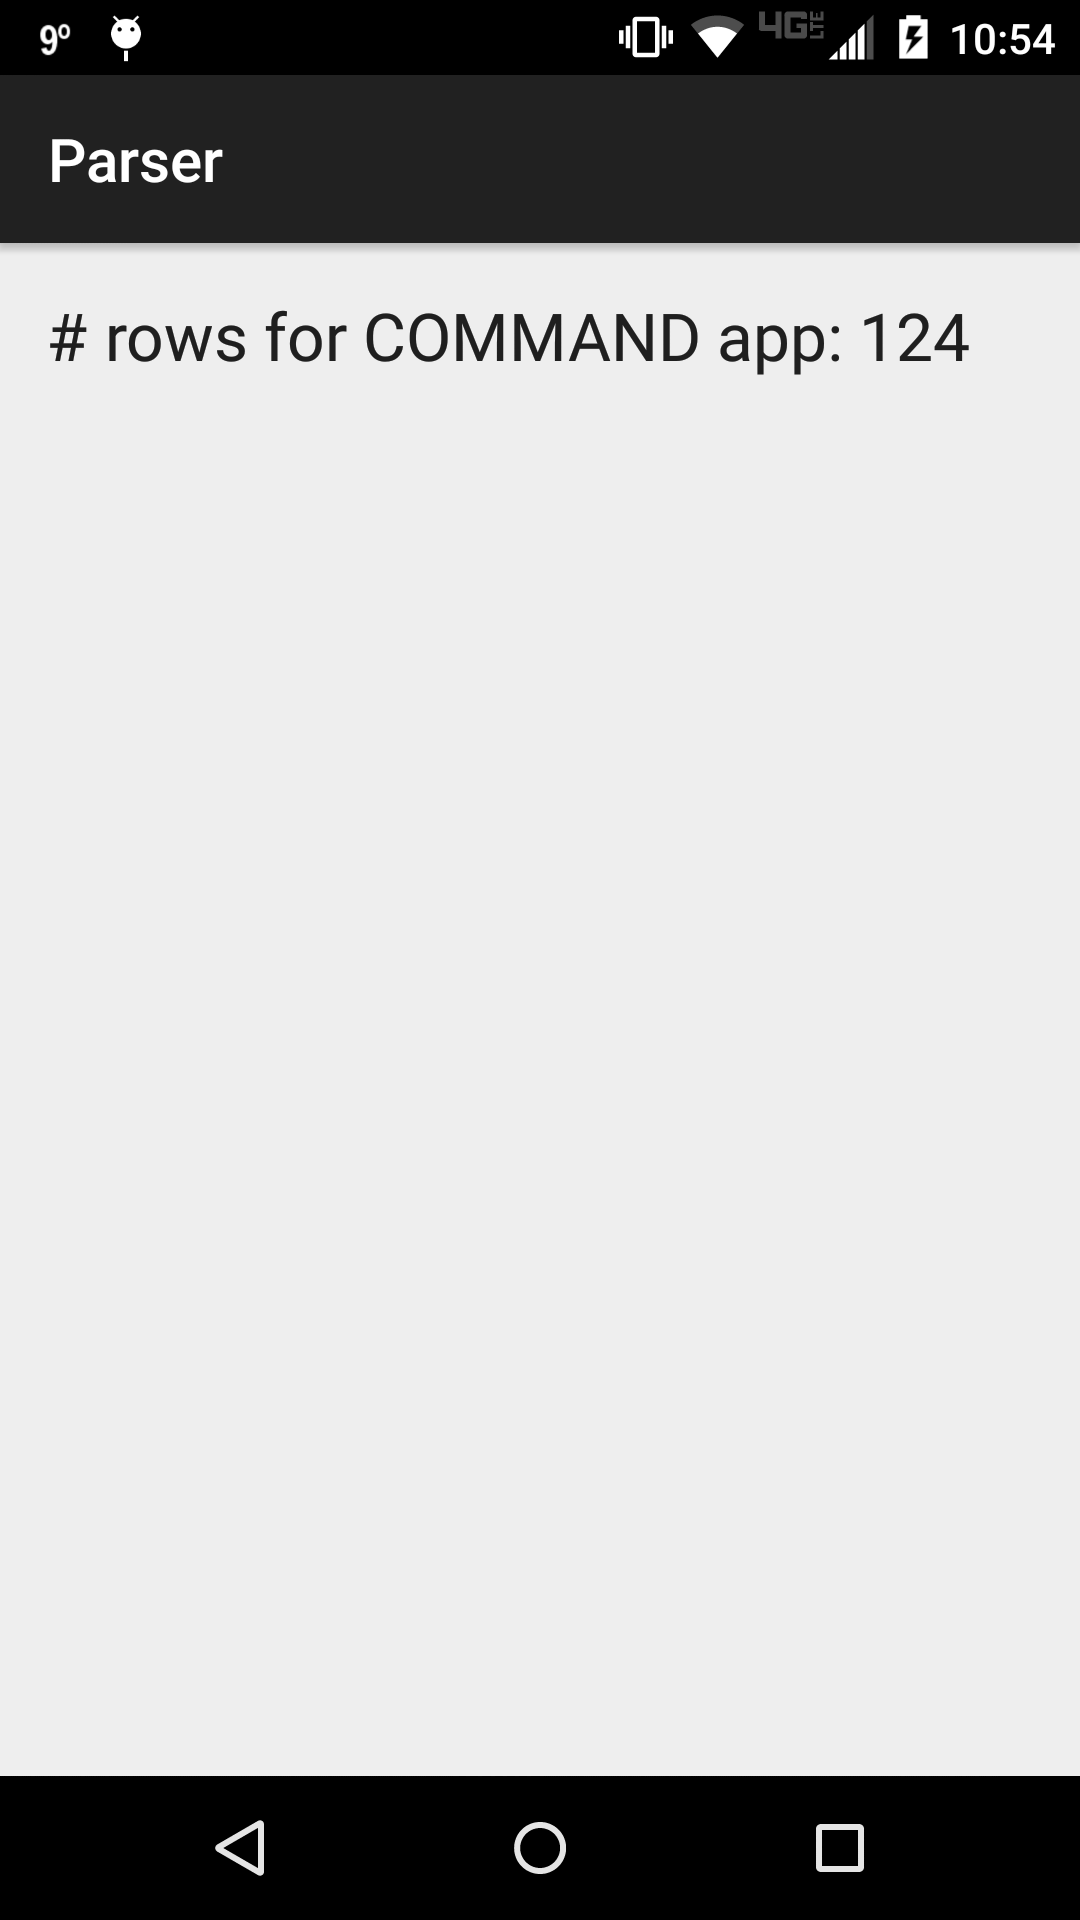
\includegraphics[width=\columnwidth,scale=0.5]{images/neitherHavePerm}
	\caption{Android content provider accessed without permission}
	\label{fig:neitherHavePerm}
\end{minipage}
\end{figure}
\subsubsection{PoC case 3 for permission control} COMMAND has associated permission, Parser has not requested said permission. We see in Figure~\ref{fig:didNotRequestPermission} that, causes a permission denial error which is what we expected.
\begin{figure}[tb]
\centering
	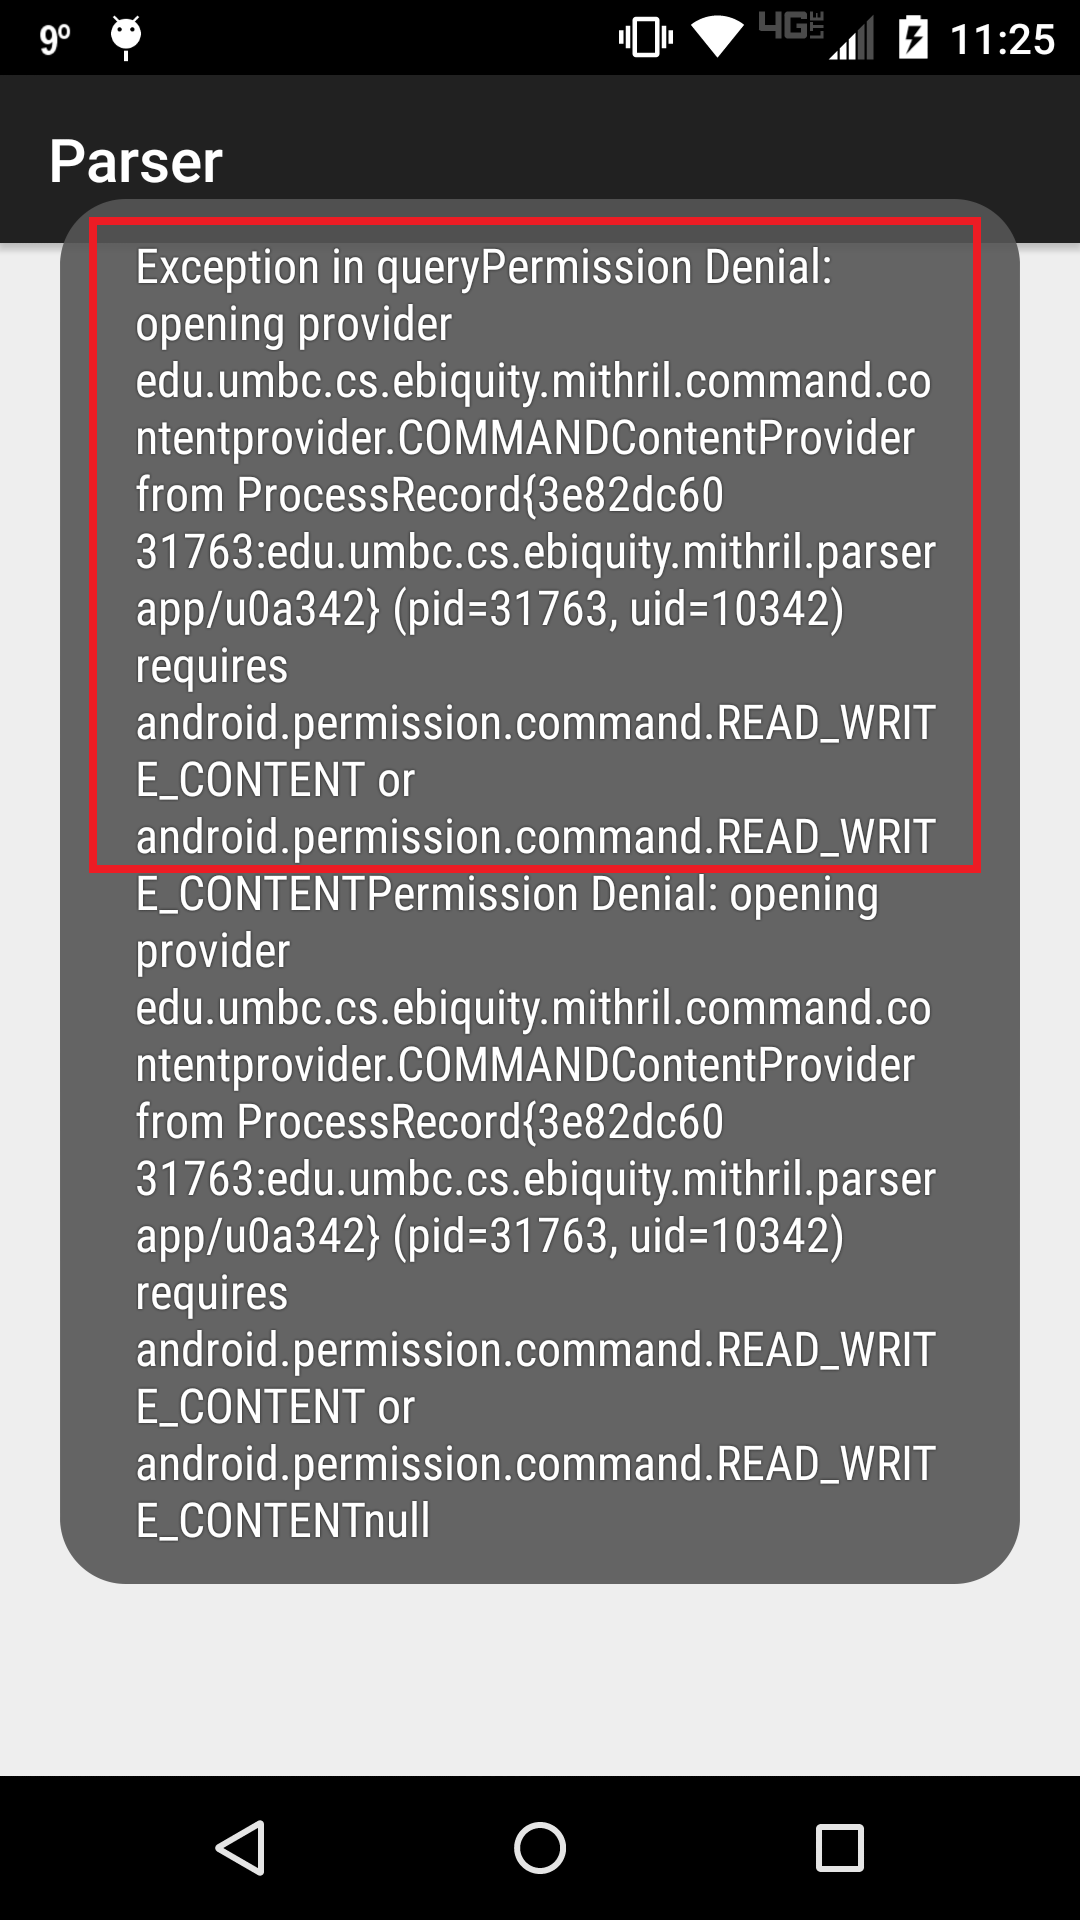
\includegraphics[scale=0.18]{images/didNotRequestPermission}
	\caption{Android content provider permission denial}
	\label{fig:didNotRequestPermission}
\end{figure}
\subsubsection{PoC case 4 for permission control} COMMAND has no associated permission in the system, Parser has requested an unknown permission. In this case there is a potential of data leakage happening on the phone as the custom content provider is not protected.

The PoC proves that there is no difference from user perspective between an app which has a content provider with proper protection and an app which does not have such access control implemented. This is because in both cases the user does not see any error on the phone and safely assumes that their data is safe. This means user data can potentially leak without user's knowledge. We ran our analysis on a set of 1500 randomly selected applications with a mix of popular applications like Facebook, GMail, Instagram as well as less popular and unknown apps like Expense Manager, Call App etc. Our system found 150 applications with content provider marked as exported=``true'' and no associated permission for the provider. Therefore about 10\% of apps have this potential loophole but we wanted to find out if we could change an app to leak it's data. 

This led to our second set of experiments trying to determine, if the apps had incorporated additional protection apart from the standard Android permission mechanisms. For these experiments we used the Facebook app and the Google Fit app. We removed all permissions associated with the providers on both the apps. We also set all the providers' exported setting to true.

\subsection{Scenario 2: App checks for signatures} Upon installation the repackaged Google fit app immediately crashed and kept on crashing every time we tried to use it. Therefore, in order to figure out the issue we used logcat, the Android logging system that provides a mechanism for collecting and viewing system debug output. We discovered from logcat messages that the Google Fit app had included an additional check on the app key signature and it simply crashed because the signature is detected as unknown. You can see the error in Figure~\ref{fig:GoogleProtections}.

\begin{figure}[tb]
\centering
	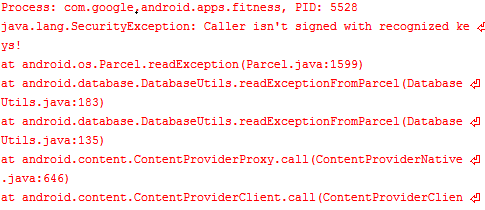
\includegraphics[width=\columnwidth]{images/GoogleProtections}
	\caption{Google Fit app checks for certificate signatures}
	\label{fig:GoogleProtections}
\end{figure}

\begin{figure}[tb]
\centering
	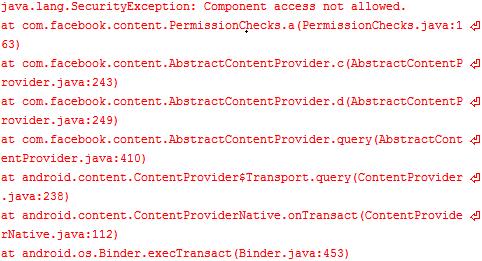
\includegraphics[width=\columnwidth]{images/FBProtections}
	\caption{Facebook checks controls access to it's component}
	\label{fig:FBProtections}
\end{figure}

\subsection{Scenario 3: App manages access control to it's components} For this case we used a repackaged Facebook app. We observed that the app never crashed and worked like a normal Facebook app. However, when we tried to access the app's content provider it blocked our attempts and you can see in Figure~\ref{fig:FBProtections} that Facebook controls access to it's own component using a custom protection mechanism. Therefore, app developers are clearly detecting such issues on their apps but not always.

\begin{figure}[tb]
\centering
	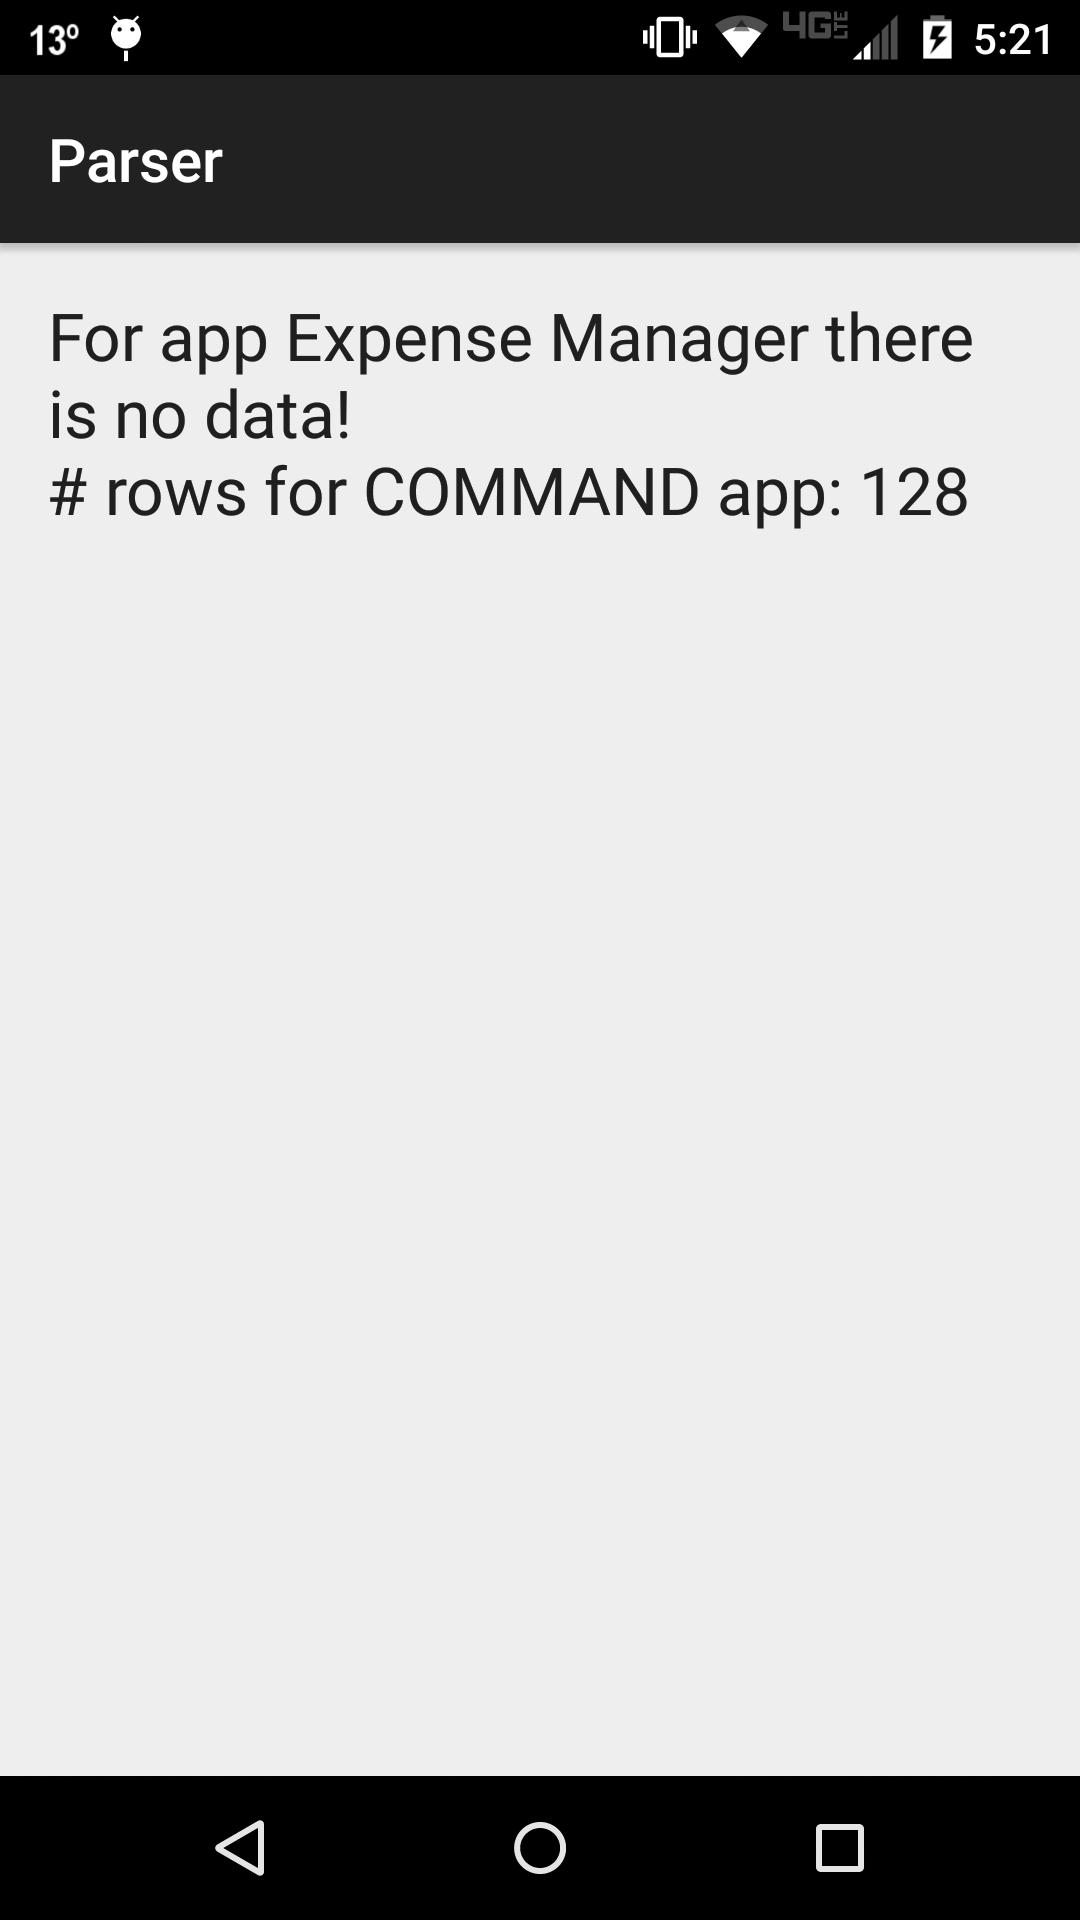
\includegraphics[scale=0.12]{images/nochecks}
	\caption{No check points were found on a less popular app}
	\label{fig:nochecks}
\end{figure}

\subsection{Scenario 4: Potentially vulnerable app} We found at least one app called Expense Management from our random sample set that allowed us access to it's content provider. However, we did not know the complete URI for the app's content provider. Therefore we had to make guesses. We repackaged this app too and following the same process as the previous apps, we observed that it did not implement any checkpoints. Also it doesn't cause any errors as we saw in the above-mentioned scenarios. You can see in Figure~\ref{fig:nochecks}, that our query did not return any data but that was because the app wasn't writing it's data to it's database. We are still investigating other apps for a potential breach that could lead to a full fledged exploit. We are currently processing more apps to find out if they include such checks as encoded by popular apps from Google or Facebook. This processing takes a long time because we have to manually find the databases on the phone using a rooted phone and a SQLite explorer app. Thereafter, we have to make guesses for patterns that apps might have used in their content provider code. There are commonly used patterns like `\#' that can be used as a part of the URI. Such a generated URI can then be used to call the content provider and obtain access to the data. We are trying to use such patterns to find out apps which have such a vulnerability.
\section{Related Work}
\label{RelatedWork}

Significant research has been done on predicting users' preferences
for
permission-granting~\cite{Benisch2011,Sadeh2009,lin2014soups,liu2014www}.
We build on this work and make the assumption that it is (or soon will
be) possible to fairly accurately create user permission choices on
Android devices. Our research goal differs in three ways. First, we
define policy rules for users which may allow, deny or allow with
caveat specific permissions depending on the user context. Second, we
are not trying to show that it is possible to learn a user's policy
from scratch but rather we are agreeing with their observation that it
is possible to use privacy profiles to define or group user
preferences~\cite{liu2014www}. Instead we are trying to show that
given user feedback it is possible to reach an individual user's
``perfect'' policy with a certain probability. Third, we are exploring
ways to include app provenance information, API usage and observed
mobile behavior~\cite{enck2010taintdroid} to compute metrics that will
accurately predict the trustworthiness of an app.

\hl{
Playdrone : Crawls Playstore- how playstore evolved - source code analysis of library usage - similar app detection-secret authentication key storage (can be found by decompilation)
(1) native libraries are heavily used by popular Android applications, limiting the benefits of Java portability and the ability of Android server overloading systems to run these applications, (2) 25\% of Google Play is duplicative application content, and (3) Android applications contain thousands of leaked secret authentication keys which

Andradar : First, we can discover malicious applications in alternative markets, second, we can expose app distribution strategies used by malware developers, and third, we can monitor how different markets react to new malware. To identify and track malicious apps still available in a number of alternative app markets.

Android Security : discuss the Android security enforcement mechanisms, threats to the existing security enforcements and related issues, malware growth timeline between 2010 and 2014, and stealth techniques employed by the malware authors, in addition to the existing detection methods. This review gives an insight into the strengths and shortcomings of the known research methodologies and provides a platform, to the researchers and practitioners, toward proposing the next-generation Android security, analysis, and malware detection techniques.

ANDRUBIS:, a fully automated, publicly available and comprehensive analysis system for Android apps. ANDRUBIS combines static analysis with dynamic analysis on both Dalvik VM and system level, as well as several stimulation techniques to increase code coverage. 

changes in the malware threat landscape and trends amongst goodware developers. Dynamic code loading, previously used as an indicator for malicious behavior, is especially gaining popularity amongst goodware App analysis for astma!!

App behavior against description CHABADA tool clustering apps by description topics, and identifying outliers
by API usage within each cluster, our CHABADA approach effectively
identifies applications whose behavior would be unexpected
given their description.
Recommendations for the Android ecosystem}

author et.al. developed a formal Android permission model to analyze the permission protocol used using Alloy. Using Alloy analyzer, they reasoned over the model to detect possible vulnerabilities in the protocol. It also generated counter examples which can possibly exploit the vulnerabilities in the protocol. Their work could detect a vulnerability in which an application with normal security level permission was able to access another application's dangerous level custom permission given the following conditions. First, both the permission names are the same and second the application with lesser security level is installed first. But we differentiate from them such that instead on just focusing on

\section{Conclusions}
\label{concl}

\section{Acknowledgments}
Support for this work was provided by NSF grant 0910838, MURI award FA9550-08-1-0265 from the Air Force Office of Scientific Research.
% The following two commands are all you need in the
% initial runs of your .tex file to
% produce the bibliography for the citations in your paper.
\bibliographystyle{abbrv}
\bibliography{bibliography}  % sigproc.bib is the name of the Bibliography in this case
@online {Engadget_market_share,
  author = {Christopher Trout},
  title = {Android still the dominant mobile OS with 1 billion active users},
  year = 2014,
  url = {http://www.engadget.com/2014/06/25/google-io-2014-by-the-numbers/},
  urldate = {2014-06-25}
}
@online {Online_App_Stores,
  author = {Ryan Chang},
  title = {10 Alternative Android App Stores},
  year = 2014,
  url = {http://code.tutsplus.com/articles/10-alternative-android-app-stores--cms-20999},
  urldate = {2014-01-08}
}
@online {Android_app_number,
  author = {Statista},
  title = {Number of available applications in the Google Play Store from December 2009 to July 2015},
  year = 2015,
  url = {http://www.statista.com/statistics/266210/number-of-available-applications-in-the-google-play-store/},
  urldate = {2015-11-29}
}

% You must have a proper ".bib" file
%  and remember to run:
% latex bibtex latex latex
% to resolve all references
%
% ACM needs 'a single self-contained file'!
%
% That's all folks!

\end{document}